\paragraph*{High inertial effects :}
We now turn our attention to the high inertial regime for which we set $Ga =100$.
In this situation it is expected that the presence of wake change completely the flow behavior. 
\begin{figure}[h!]
    \centering
    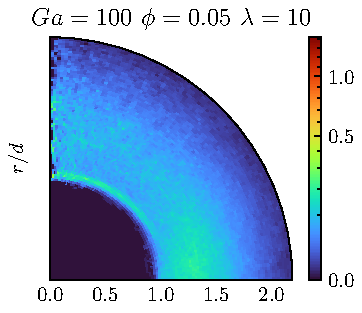
\includegraphics[height=0.2\textwidth]{image/HOMOGENEOUS_NEW/Dist/Pnst_l_10_Ga_100_PHI_0_05.pdf}
    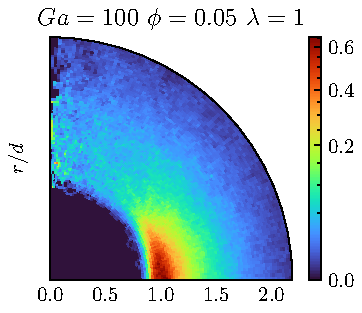
\includegraphics[height=0.2\textwidth]{image/HOMOGENEOUS_NEW/Dist/Pnst_l_1_Ga_100_PHI_0_05.pdf}
    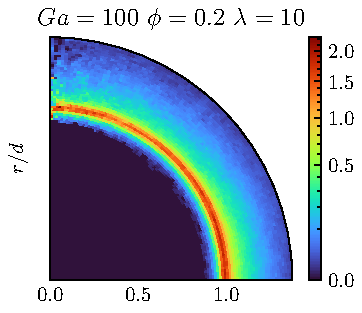
\includegraphics[height=0.2\textwidth]{image/HOMOGENEOUS_NEW/Dist/Pnst_l_10_Ga_100_PHI_0_2.pdf}
    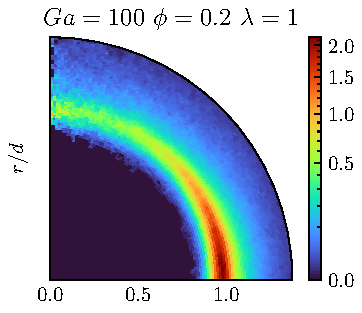
\includegraphics[height=0.2\textwidth]{image/HOMOGENEOUS_NEW/Dist/Pnst_l_1_Ga_100_PHI_0_2.pdf}
    \caption{Histogram of the probability density function $P_\text{nst}$ at high inertial effect $Ga = 100$.
    (left) Low volume fraction cases $\phi=0.05$ for $\lambda = 1,10$.
    (right) High volume fraction cases $\phi=0.1$ for $\lambda = 1,10$ }
    \label{fig:Pnst_high_Ga}
\end{figure}
As expected, if we compare \ref{fig:Pnst_high_Ga} (right) with their corresponding cases from \ref{fig:Pnst_low_Ga} (right) we observe that the nearest PDF becomes even more concentrated at contact of the particles for $Ga=100$.
In general, if we compare all PDF from the low inertial cases to these, the striking difference is the presence of anisotropy in \ref{fig:Pnst_high_Ga}. 
Especially, even within the high inertial cases we can notice that the PDF is even more concentrated on the sides for $\lambda = 1$. 
Consequently, it is clear that the PDF concentration on the side increase for increasing $Ga$ and for low viscosity ratio. 
Regarding, the volume fraction it is found to decrease the anisotropy but makes the particles closer. 

To illustrate the influence of the viscosity ratio on the microstructure \ref{fig:images} displays snapshots of two DNS at $\phi = 0.05$ and $Ga = 100$. 
As predicted by $P_\text{nst}$ in \ref{fig:Pnst_high_Ga} we observe strong layers of droplets for $\lambda = 1$ in opposition to the viscous droplets which are more evenly dispersed. 
As discussed in \citet{zhang2021three}, rising pairs of spherical bubbles reach a stable side-by-side configuration which tends to generate horizontal clusters. 
\begin{figure}[h!]
    \centering
    % 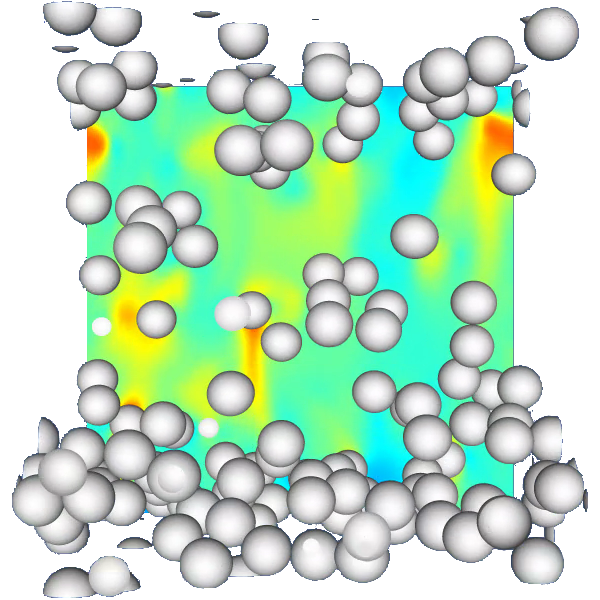
\includegraphics[width=0.3\textwidth]{image/HOMOGENEOUS_NEW/P_PHI_5_l_01_Ga_100.png}
    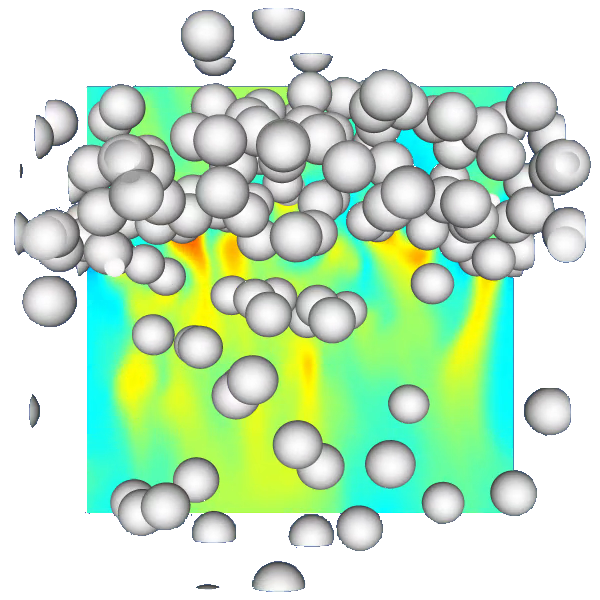
\includegraphics[width=0.35\textwidth]{image/HOMOGENEOUS_NEW/P_PHI_5_l_10_Ga_100.png}
    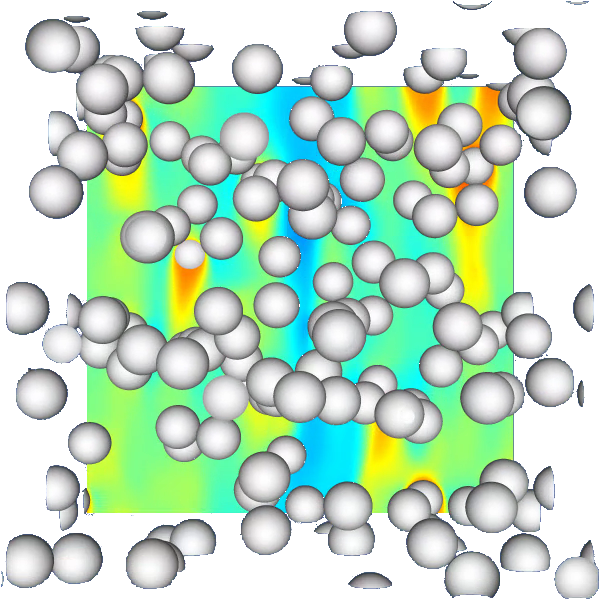
\includegraphics[width=0.35\textwidth]{image/HOMOGENEOUS_NEW/P_PHI_5_l_1_Ga_100.png}
    \caption{Snapshot of a simulation at $t^* = 150$ for $\phi=0.05$ and $Ga=100$.
    Color map : values of the vertical component of the velocity, field on the vertical plane defined by the equation $z=0$. 
    (left)  $\lambda = 1$.
    (right)  $\lambda = 10$.
    }
    \label{fig:images}
\end{figure}
Clearly, the viscosity ratio appears to maintain a significant distance between particles, which prevent the creation of structures such as droplets layers.
This might be the cause of a higher vorticity around the viscous droplets.   
In fact in \ref{fig:images} we can observe horizontal raft of droplets or droplets rising side-by-side, but this effect is clearly not as pronounce as for the iso-viscous case. 
Nevertheless, we can observe on \ref{fig:images}(left) that the length between the layers is roughly equal to the length of the numerical domain. 
Indeed, only one layer of droplets is present in the domain. 
Therefore, at this stage it is hard to known for sure if the current microstructure is constrained by the size of the numerical domain, or if it is well representative of the actual microstructure that we would obtain in an infinite non-periodic domain. 
Consequently, in all rigor DNS in a larger domain would be required to evaluate the microstructure dependence on the domain size. 
It is clear that DNS in a larger domain with the same dimensionless parameters are expensive therefore it has not been conducted in this study. 
One might argue that the layers appear due to collective effect constrained by the size of the box, and that it would not arise in a greater box. 
However, in \citet{legendre2003hydrodynamic} they study the interaction between a pair of bubbles rising side-by-side. 
They stipulate that for two bubbles at moderate Reynolds number $50-100$, the interaction forces is found to be repulsive, while it is attractive or null for higher Reynolds. 
In our case it is reasonable to think that such pair attraction / repulsion mechanisms might also drive the clustering mechanism for the higher \textit{Galileo} cases at $\lambda = 1$.
Therefore, we might expect that horizontal layers such as the one observed in \ref{fig:images} (left) still remain for lager boxes since they are more probability due to pairwise interactions mechanism and not collective effect. 
Consequently, the only conclusion from  \ref{fig:images} that we are able to make is : more cluster are formed at $\lambda =1$ than at $\lambda = 10$, however we cannot be sure that the cluster are realistic in the former case. 

A last remark is that while these pair statistic represent only nearest pair interaction, the clustering or not graphs only represent the interaction witht the nearest neighbor. 
Therefore, in \ref{fig:Pnst_high_Ga} for example it must be understood that we, in theory are only able to predict \textit{pair clustering} and not the whole cluster shown \ref{fig:images}.
However, as it will be demonstrated in the next section, pairs interactions last for a finite amount of time. 
Consequently, structure observed on \ref{fig:Pnst_high_Ga} are actually representative of macroscopic cluster such as in \ref{fig:images}. 


\subsection{Nearest radial distribution function }

Although, \ref{fig:Pnst_high_Ga} and \ref{fig:Pnst_low_Ga} give a good representation of the particle pair azimuthal distribution, it is hard to inspect in details the radial distribution.
Therefore, in \ref{fig:Pr}  we plotted the radial distribution $P_\text{nst}(r)$ for two different viscosity ratios and multiples \textit{Galileo} numbers in terms of the dimensionless distance $(r - d)/d_p$ where $d_p$ is the mean particle distance defined as $d_p = n_p^{-1/3}$.  
For a random isotropic distribution of hard spheres it is possible to derive a theoretical prediction for $P_\text{nst}(|\textbf{r}|)$ obtained in limiting cases. 
Indeed, it is shown in \citet{zhang2021ensemble} that for a dilute random arrangement of particle the probability density of the nearest PDF reads as, 
\begin{equation}
    P_\text{nst}^\text{th}(\textbf{x},t,r) = n_p \exp[{-4 \pi n_p(\textbf{x},t) (r^3 - d^3)/3}].
    \label{eq:Pnst_dilute}
\end{equation}
where $P_\text{nst}(\textbf{x},t,r) = \int_0^\infty P_\text{nst}(\textbf{x},\textbf{r},t,a) da$.
It must be understood that this formula is accurate only at $\mathcal{O}(\phi)$ therefore in most of our cases it is not supposed to represent the real distribution.
Additionally, the hard sphere model differ considerably form the droplets pair distribution since in the latter case $P_\text{nst}^\text{th} = 0$ for $r<d$ while in our case the distribution remain finite since particles might inter-penetrate. 
However, it remains valuable to utilize this theoretical probability density function for comparative purposes. 

\begin{figure}[h!]
    \centering
    % 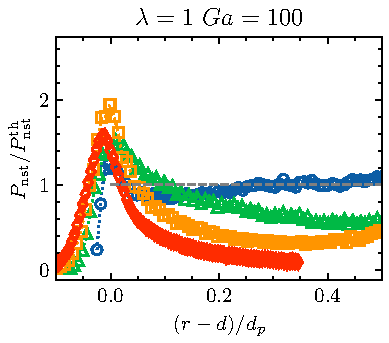
\includegraphics[height=0.3\textwidth]{image/HOMOGENEOUS_NEW/Dist/Pr_l_1_Ga_100.pdf}
    % 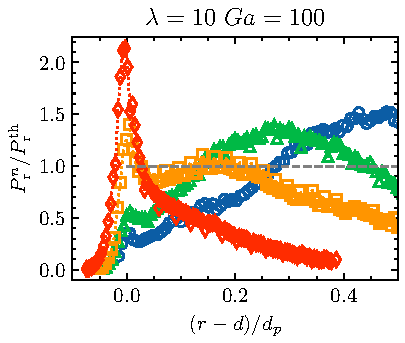
\includegraphics[height=0.3\textwidth]{image/HOMOGENEOUS_NEW/Dist/Pr_l_10_Ga_100.pdf}
    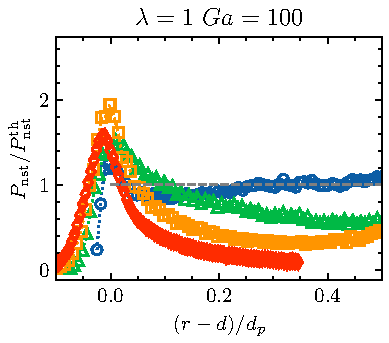
\includegraphics[height=0.3\textwidth]{image/HOMOGENEOUS_NEW/Dist/Pr_l_1_Ga_100.pdf}
    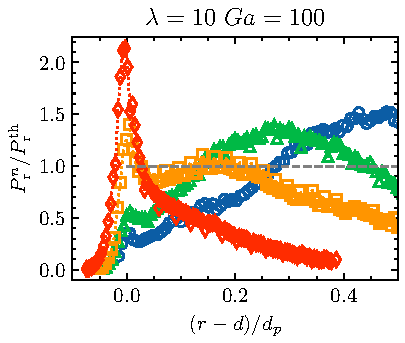
\includegraphics[height=0.3\textwidth]{image/HOMOGENEOUS_NEW/Dist/Pr_l_10_Ga_100.pdf}
    \caption{Radial probability density function $P_\text{nst}(|r|)$ divided by the theoretical distribution \ref{eq:Pnst_dilute} in terms of the dimensionless distance $(r-d)/d_p$ where, $d_p = n_p^{-1/3}$, for  $Ga = 100$.
    (left)  $\lambda = 1$.
    (right) $\lambda = 10$.
    ($\pmb\bigcirc$) $\phi = 0.01$; ($\pmb\triangle$) $ \phi = 0.05$; ($\pmb\square$) $\phi = 0.1$ ($\pmb\lozenge$) $\phi = 0.2$.
    For $r<d$ we arbitrarily set $P_\text{nst}^\text{th} = 1$ so that the distribution can be visualized.
    }
    \label{fig:Pr}
\end{figure}
The radial distribution seem concentrated in different zones with varying \textit{Galileo} number when $\lambda = 1$, see \ref{fig:Pr}(left), while the distribution seem rather unchanged with multiples \textit{Galileo} numbers for $\lambda = 10$ \ref{fig:images}(right). 
In both cases the radial distribution does not follow the random hard sphere distribution defined by \ref{eq:Pnst_dilute}. 
Far from the particle the distribution seem tangent to it 
It is clear that when inertial effects are strong, the viscosity ratio $\lambda$ has an important impact on the radial distribution. 
Indeed, we can notice the remarkable difference between \ref{fig:Pr}(left) and  \ref{fig:Pr}(right) at $Ga = 100$ ($\lozenge$ symbols). 
For $\lambda = 1$ the distribution at $Ga = 100$ is high at the contact of the particles $(r-d)/d_p = 0$. 
In fact, it is not surprising when considering the high particle density zone formed by the cluster, see \ref{fig:images}(left). 
In opposition, for $\lambda  = 10$ the radial distribution it is completely different, the particles are in averaged further away form each other, as it could be predicted from \ref{fig:images}(right).
Additionally, the effect of the \textit{Galileo} number on $P_\text{nst}(r)$ doesn't seem important contrasting with the low viscosity ratio cases where it has a major influence.  
Although, we choose a small \textit{Bond} number it is clear from \ref{fig:Pr} that the particles inter penetrate with each other as witnesses by the non vanishing value of $P_\text{nst}$ for $r-d<0$.

In short, we observed that both, the radial and azimuthal distribution were affected by the inertial effect measured by the \textit{Galileo} number. 
The major effect coming with high inertia is the generation of strong anisotropy in the particle pair distribution. 
Regarding the viscosity ratio, it has a strong impact on the emulsion distribution, however, this is only true at high $Ga$ whereas at low $Ga$ the change in viscosity ratio has no notable impact. 
Furthermore, low viscosity ratio generate anisotropy in the distribution.  
Additionally, it is seen that the particle distribution gets more concentrated at the contact of the test sphere, but only for $\lambda = 1$. 


\subsection{Macroscopic modeling of the microstructure}

Up to now we provided a 2D or 1D way to visualize the microstructure. 
Now we would like to provide a more quantitative description of the microstructure, eventually a tensor quantity might be sufficient to describe the microstructure for all our cases. 
Following \citet{zhang2023evolution} we chose to describe the microstructure of the flow using the second moment of the nearest pair probability density function, namely,
\begin{equation}
    \textbf{R}(\textbf{x},t) =\frac{1}{n_p(\textbf{x},t)} 
    \int_0^\infty 
    \int_{\mathbb{R}^3} \textbf{rr} P_\text{nst}(\textbf{x},\textbf{r},t,a) d\textbf{r} da.
    \label{eq:R}
\end{equation}
This tensor is in fact the standard deviation on $\textbf{r}$ of the nearest particle pair distribution. 
It measures the spread of particle in a given direction. 
Note that such a quantity is computable only because $\lim_{|\textbf{r}|\to \infty} P(\textbf{x},\textbf{r},t,a) = 0$ which enable the integral of \ref{eq:R} to converge. 
Which is not the case for classic pair distribution, this is why we believe the nearest particle statistics is more powerful. 
Since our objective is to point out the anisotropy of the microstructure we are interested in the Deviatoric part of this tensor, namely, 
\begin{equation*}
    \textbf{A}(\textbf{x},t) = \textbf{R}(\textbf{x},t) - \frac{1}{3} [\textbf{R}(\textbf{x},t) : \textbf{I}] \textbf{I}.
\end{equation*}
The tensor $\textbf{R}(\textbf{x},t)$ permits us to measure the mean square distance between a particle and its nearest neighbor in average in the three dimension of space. 
Therefore, $\textbf{A}(\textbf{x},t)$ is the difference of the mean square distance between a particle and its nearest neighbor with the radial mean square distance $\textbf{R}:\textbf{I}$. 
So it must be understood that for an isotropic suspension $A_{xx} = A_{xx} = 0$. 
On a situation such as in \ref{fig:images} (left) it is clear that $A_{yy} < 0 < A_{xx}\approx A_{zz}$ since a particle is more likely to have its nearest neighbor on the side rather than on the verticals. 
For a better interpretation of the following results it might be of interest to compute the distance $r_m$, which is the mean distance to the nearest neighboring particle in a random distribution of hard sphere described by, \ref{eq:Pnst_dilute}. 
By direct integration we find, 
\begin{equation*}
    r_m^2 /d^2
    = \textbf{I}:\textbf{R}(\textbf{x},t)/d^2
    = {{4^{{{2}\over{3}}}\,\Gamma\left({{5}\over{3}} , 8\,\phi\right)
    \,e^{8\,\phi}}\over{2^{{{10}\over{3}}}\,\phi^{{{2}\over{3}}}}}
\end{equation*}
where $\Gamma(z,a) = \int_a^\infty t^{z-1} e^{-t} dt$ is the upper incomplete gamma function. 
This mean that for any particle in the flow in a hard sphere distribution, the nearest neighbor is in average at a distance of $r_m$ from a given particle.  

\begin{figure}[h!]
    \centering
    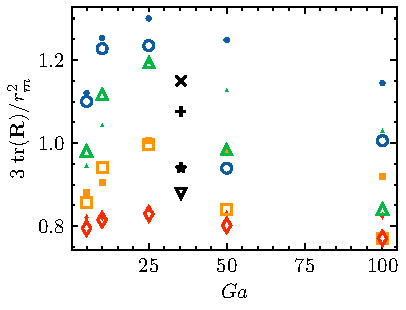
\includegraphics[height=0.3\textwidth]{image/HOMOGENEOUS_NEW/PA/trR.pdf}
    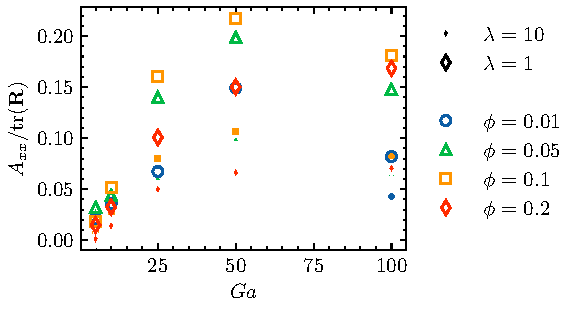
\includegraphics[height=0.3\textwidth]{image/HOMOGENEOUS_NEW/PA/Axx.pdf}
    \caption{
        (left) Trace of the second moment of the probability density function $P_\text{nst}(\textbf{r})$ divided by the square diameter of the particles $d^2$. 
        (right) vertical components of the anisotropy tensor divided by the trace of the second moment of the probability density function.
    ($\pmb\bigcirc$) $\phi = 0.01$; ($\pmb\triangle$) $ \phi = 0.05$; ($\pmb\square$) $\phi = 0.1$ ($\pmb\lozenge$) $\phi = 0.2$.
    The hollow symbols correspond to $\lambda = 1$, the filled symbols to $\lambda = 10$.
    For $r<d$ we arbitrarily set $P_\text{nst}^\text{th} = 1$ so that the distribution can be visualized.
    Black symbols represent the results of \citet{zhang2023evolution} for hard sphere suspension with $\phi = 0.016,0.056,0.134,0.262$  %$\phi = 0.0168,0.0565,0.1341,0.2622$ 
    corresponding to $\pmb\times,\pmb +, \pmb\star , \pmb\triangledown$, respectively.
    }
    \label{fig:A}
\end{figure}
\ref{fig:A} (left) displays the value of the mean square distance : $\textbf{I}:\textbf{R}/r_m^2$, between nearest neighbors for all our numerical cases. 
To help comprehension, it is helpful to note that the simulation denoted by a \textcolor{col1}{$\pmb\circ$} in \ref{fig:A} (left), corresponding to $\lambda = 1$, $Ga = 100$ and $\phi = 0.01$ has a value of $\textbf{I}:\textbf{R}/r_m^2 = 1$, which is consistent with the quasi hard sphere distribution obtained for this case in \ref{fig:Pr} (left). 
It is clear from the graph that the mean square distance is mainly dependent on the volume fraction. 
We observe that $\textbf{I}:\textbf{R}/r_m^2$  decrease for increasing $\phi$, which means that particles get in average closer to one another compared to a hard sphere random distribution. 
As noted by \citet{zhang2023evolution} this implies the apparition of clusters. 
The dependence on the \textit{Galileo} number is non-monotonic, the distance is increasing until $Ga = 25$ and the decreasing until $Ga = 100$.  
At rather high $Ga$ one might notice that the mean square distance for $\lambda = 1$ (hollow symbols) is lower. 
For all our DNS we observe that the distance to the nearest neighbor for iso-viscous emulsions is on average more distant for $\lambda = 10$ which is consistent with the distributions displayed \ref{fig:Pr} and the picture from \ref{fig:images}.  
On \ref{fig:A} (left) the symbols : $\pmb\star, \pmb\times,\pmb +, \pmb\triangledown$, represent the results of \citet{zhang2023evolution} for hard sphere suspension. 
As we can observe the value of $\textbf{R}:\textbf{I}$ is in average closer to $r_m^2$ than our simulation but keep the same tendency, i.e. cluster appear as the volume fraction increase. 
 
Regarding the anisotropy measure we can see on \ref{fig:A} (right) that first we have $A_{xx} \ge 0$ for nearly all our cases, meaning that globally, the emulsion is either isotropic for $A_{xx} = 0$ or with particles in average aligned on horizontally for $A_{xx} >0$. 
Then, we can see that $A_{xx}$ increase until $Ga = 50$ where we reach the maximum anisotropy, and then decrease until $Ga =100$  but remain still positive. 
Consistently with the cases\ref{fig:images} the value of the anisotropy tensor is greater for $\lambda = 1$ lower for  $\lambda = 10$.
Although, it is not quite obvious we observe a non-monotonic tendency with teh volume fraction, indeed $A_{xx}$ first increase up to a maximum value for $\phi =0.1$ (represented by \textcolor{col3}{$\pmb\square$} on \ref{fig:A} (right)) and then decrease for $\phi=0.2$ (represented by the \textcolor{col3}{$\pmb\lozenge$} symbols). 
This latter fact remains true for both volume fraction. 
It does mean that at some point in the volume fraction of droplets tends to randomize the emulsion while at moderate volume fraction it helps to gather side-by-side. 
This phenomenon of isotropisation at high $\phi$ has been reported in other studies such as in \citet{seyed2021sedimentation} for sedimentation of solid particles. 
However, at high \textit{Galileo} number it seems that this effect disappear since the values of the cases $\phi>0.05$ seems equivalent meaning that the suspension keep its anisotropy even at $\phi=0.2$. 
In short, we observed that the mean square particle distance compared to a random case were decreasing with the volume fraction, and is higher for viscous particles ($\lambda = 10$), meanwhile the Likelihood of finding a nearest neighboring particle on the horizontal is greater for $\lambda=1$ than $\lambda = 10$ and it non-monotonic with $Ga$ and $\phi$. 


\paragraph*{Bibliography : } 
Although, previous studies mainly focused on bubbles or solid particles, it is reasonable to compare the $\lambda = 1$ and $10$ cases to the former and the latter respectively. 
In \citet{bunner2002} they performed tri-periodic simulation of buoyant bubbles at $Re \approx 10-30$ depending on $\phi$, and they reported a preference  for the bubbles to be aligned horizontally, which is consistent with the potential flow theory. 
It is consistent with what we observe in \ref{fig:A} (right) since the anisotropy tensor $A_{xx}$ is clearly positive for $Ga = 25$ (which correspond roughly to $Re = 25$) for our $\lambda = 1$ cases (represented by hollow symbols). 
Here we argue that for low viscosity ratio $\lambda = 1$ and $Ga = 100$ we recover potential flow limit interactions which makes the side-by-side configuration more stable. 


For solid particles at $Ga = 144$ it is observed in \citet{shajahan2023inertial} that in the dilute regime, $\phi \approx 0.02$, verticals raft of particles are formed. 
In our case we could not observe such a phenomenon, meaning that it might arise at even higher viscosity ratio or \textit{Galileo} number. 
The latter effect is explained by the presence of a more developed wake for dilute solid particles which trap neighboring particles within the wake without repulsing it on the sides. 
In our case we observe more particles in the verticals' directions for $\lambda = 10$ than $\lambda =1$ at $Ga =100$ in \ref{fig:A}(right), since $A_{xx}$ is smaller in the former cases, see \ref{fig:A}.
Although it is not quite obvious in the results it might be the consequence of the same effects, i.e., the wake of the viscous drop might induce less side-by-side configuration. 
DNS at higher $Ga$ would be necessary to confirm or not the presence of the wake trapping effect and especially at which $\lambda$ it arises.  
In the moderately dense regime,  $0.02 < \phi \le 10$ they identified more configuration of particles situated side-by-side. 
As mentioned above even if it is less pronounce than for the iso-viscous case we indeed observe that on \ref{fig:A} (right). 


In the end \ref{fig:A} constitute a major results of this work as it quantify the microstructure with a single tensor quantity \textbf{R} for various $Ga$, $\phi$ and $\lambda$. 
From the value of \textbf{R} an approximation of the distribution $P_\text{nst-app}$ might be reconstructed assuming a certain functional form with 2 degree of freedom. 
In return this approximated distribution could be used to better solve certain theoretical problem involving the pair distribution function, (see for example, \citet{batchelor1972sedimentation}, \citep{hinch1977averaged} and \citep{zhang2021ensemble} where they compute theoretically the sedimentation velocity), instead of using a random distribution function such as \ref{eq:Pnst_dilute}, 


In the following we try to explain the origin of the striking difference between $\lambda = 1$ and $\lambda = 10$ on the particle pair distribution.
With this objective in mind, we present in the following section a meticulous analysis of the particle time of interaction, as well as study on the relative average particles' velocity fields. 
